\newpage
\section{Keyframe Animation and Interpolation}

\begin{figure}[!htb]
    \centering
    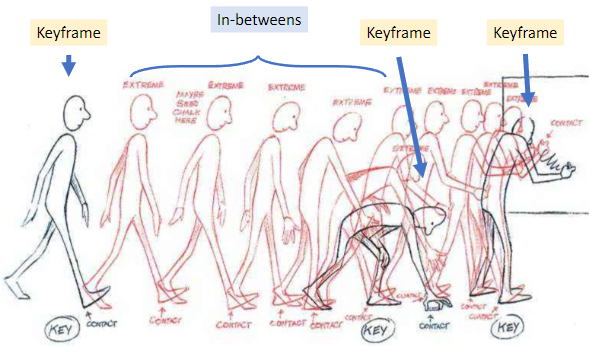
\includegraphics[width=0.618\linewidth]{pic/1054/Keyframe Animation}
    \caption{Keyframe Animation}
\end{figure}

\subsection{Interpolation}
Given a set of data pairs $D=\{ (x_i, y_i)| 0,\dots,N \}$, find a function $f(x)$ such that 
\begin{align*}
    f(x_i)=y_i,\ \forall (x_i, y_i)\in D
\end{align*}

用内插法, 而不是外插.  数值分析内容, 摸了.
\begin{itemize}
    \item Stepped Interpolation
    \item Linear Interpolation
\end{itemize}

Smoothness: 让函数值, 一阶导数, 二阶导数平滑. 

\begin{itemize}
    \item Polynomial Interpolation
    \item Spline Interpolation
    \item Cubic Splines(三次样条)
    \item Cubic Hermite Splines
    \item Hermite Basis Functions
    \item Generalization to Higher Dimensionality
\end{itemize}


龙格现象, 边缘会震荡. 所以倾向于低维.

\subsection{Interpolation of Rotations}
\begin{itemize}
    \item Interpolate parameters using (linear/cubic) splines. Rotational speed is usually not constant. 
    \item SLERP for Quaternions. Constant rotational speed, but only ``linear'' interpolation. 
    \item 四元数的贝塞尔曲线. 用 SLERP 代替线性.
\end{itemize}

一般旋转的插值, 如果关键帧设的好,其实效果都差不多. 所以其实方法都那样. 


